% Created 2019-03-07 Do 08:32
% Intended LaTeX compiler: pdflatex
\documentclass[presentation]{etp-beamer-fancy}
\usepackage[utf8]{inputenc}
\usepackage[T1]{fontenc}
\usepackage{graphicx}
\usepackage{grffile}
\usepackage{longtable}
\usepackage{wrapfig}
\usepackage{rotating}
\usepackage[normalem]{ulem}
\usepackage{amsmath}
\usepackage{textcomp}
\usepackage{amssymb}
\usepackage{capt-of}
\usepackage{hyperref}
\usepackage{physics}
\usepackage{siunitx}
\usepackage{booktabs}
\usepackage{microtype}
\usetheme{default}
\author{Michael Eliachevitch}
\date{2019-03-07}
\title{Michael's current WIP}
\subtitle{ETP B-group meeting}
\institute{ETP -- KIT}
\hypersetup{
 pdfauthor={Michael Eliachevitch},
 pdftitle={Michael's current WIP},
 pdfkeywords={},
 pdfsubject={},
 pdfcreator={Emacs 26.1 (Org mode 9.2)}, 
 pdflang={English}}
\begin{document}

\maketitle
\section*{Slides}
\label{sec:org7c4f0e0}
\begin{frame}[label={sec:org652d49d}]{Redid testing of CDC QI with full tracking}
\begin{columns}
\begin{column}{0.33\columnwidth}
\begin{center}
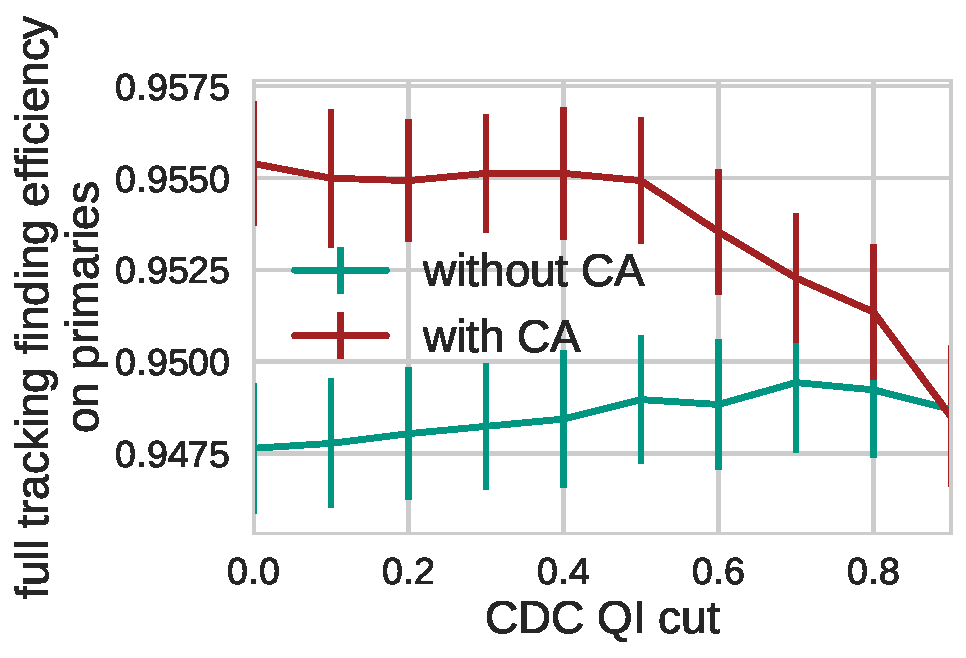
\includegraphics[width=\textwidth]{./figures/full-finding-efficiency-by-cdc-qi-cut.pdf}
\end{center}
\begin{center}
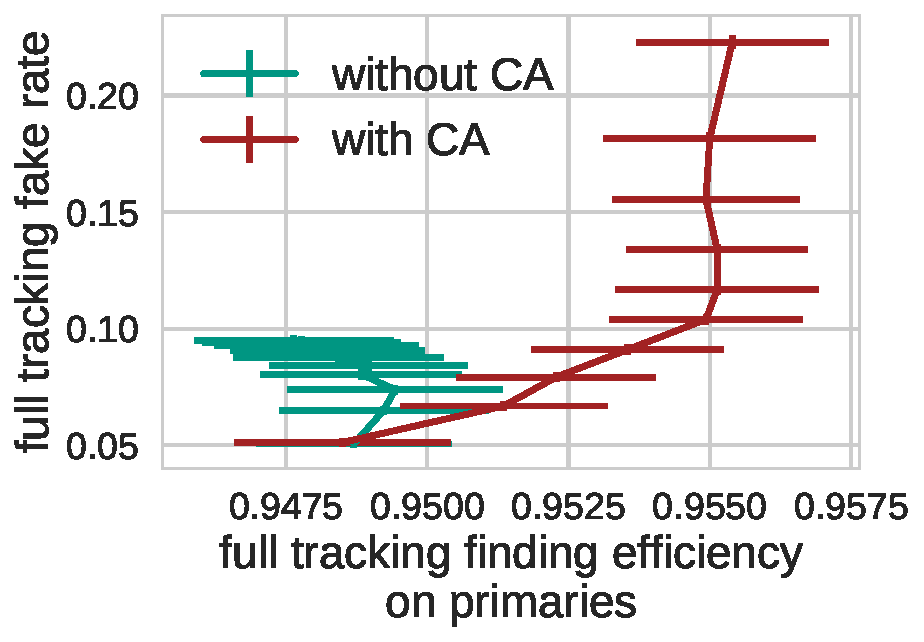
\includegraphics[width=\textwidth]{./figures/full-qi_roc_curve.pdf}
\end{center}
\end{column}
\begin{column}{0.33\columnwidth}
\begin{center}
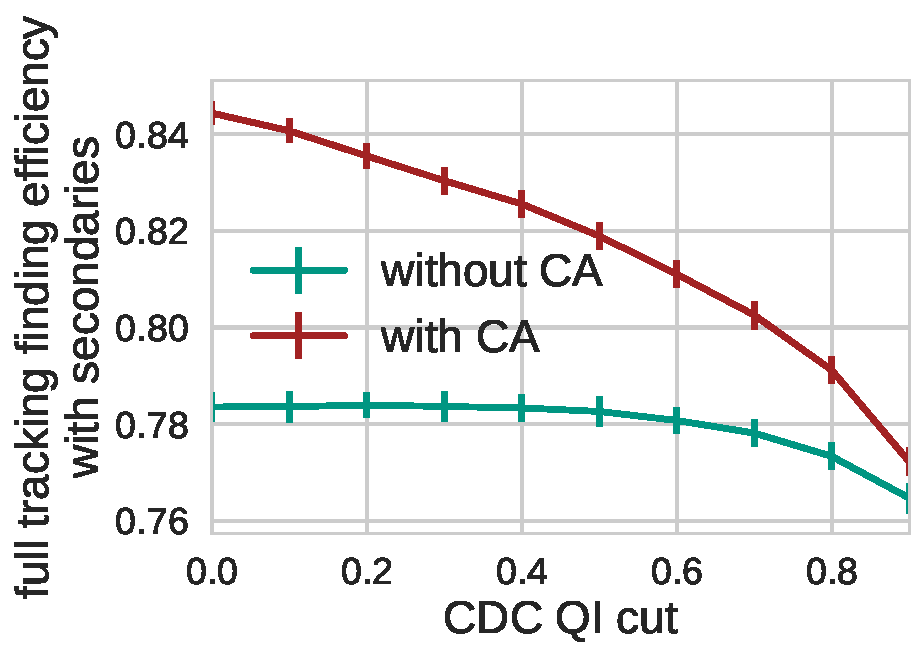
\includegraphics[width=\textwidth]{./figures/full-finding-efficiency-secondaries-by-cdc-qi-cut.pdf}
\end{center}
\end{column}
\end{columns}
\end{frame}

\begin{frame}[label={sec:org7261e34}]{Validation for PR to check for hidden changes}
\begin{center}
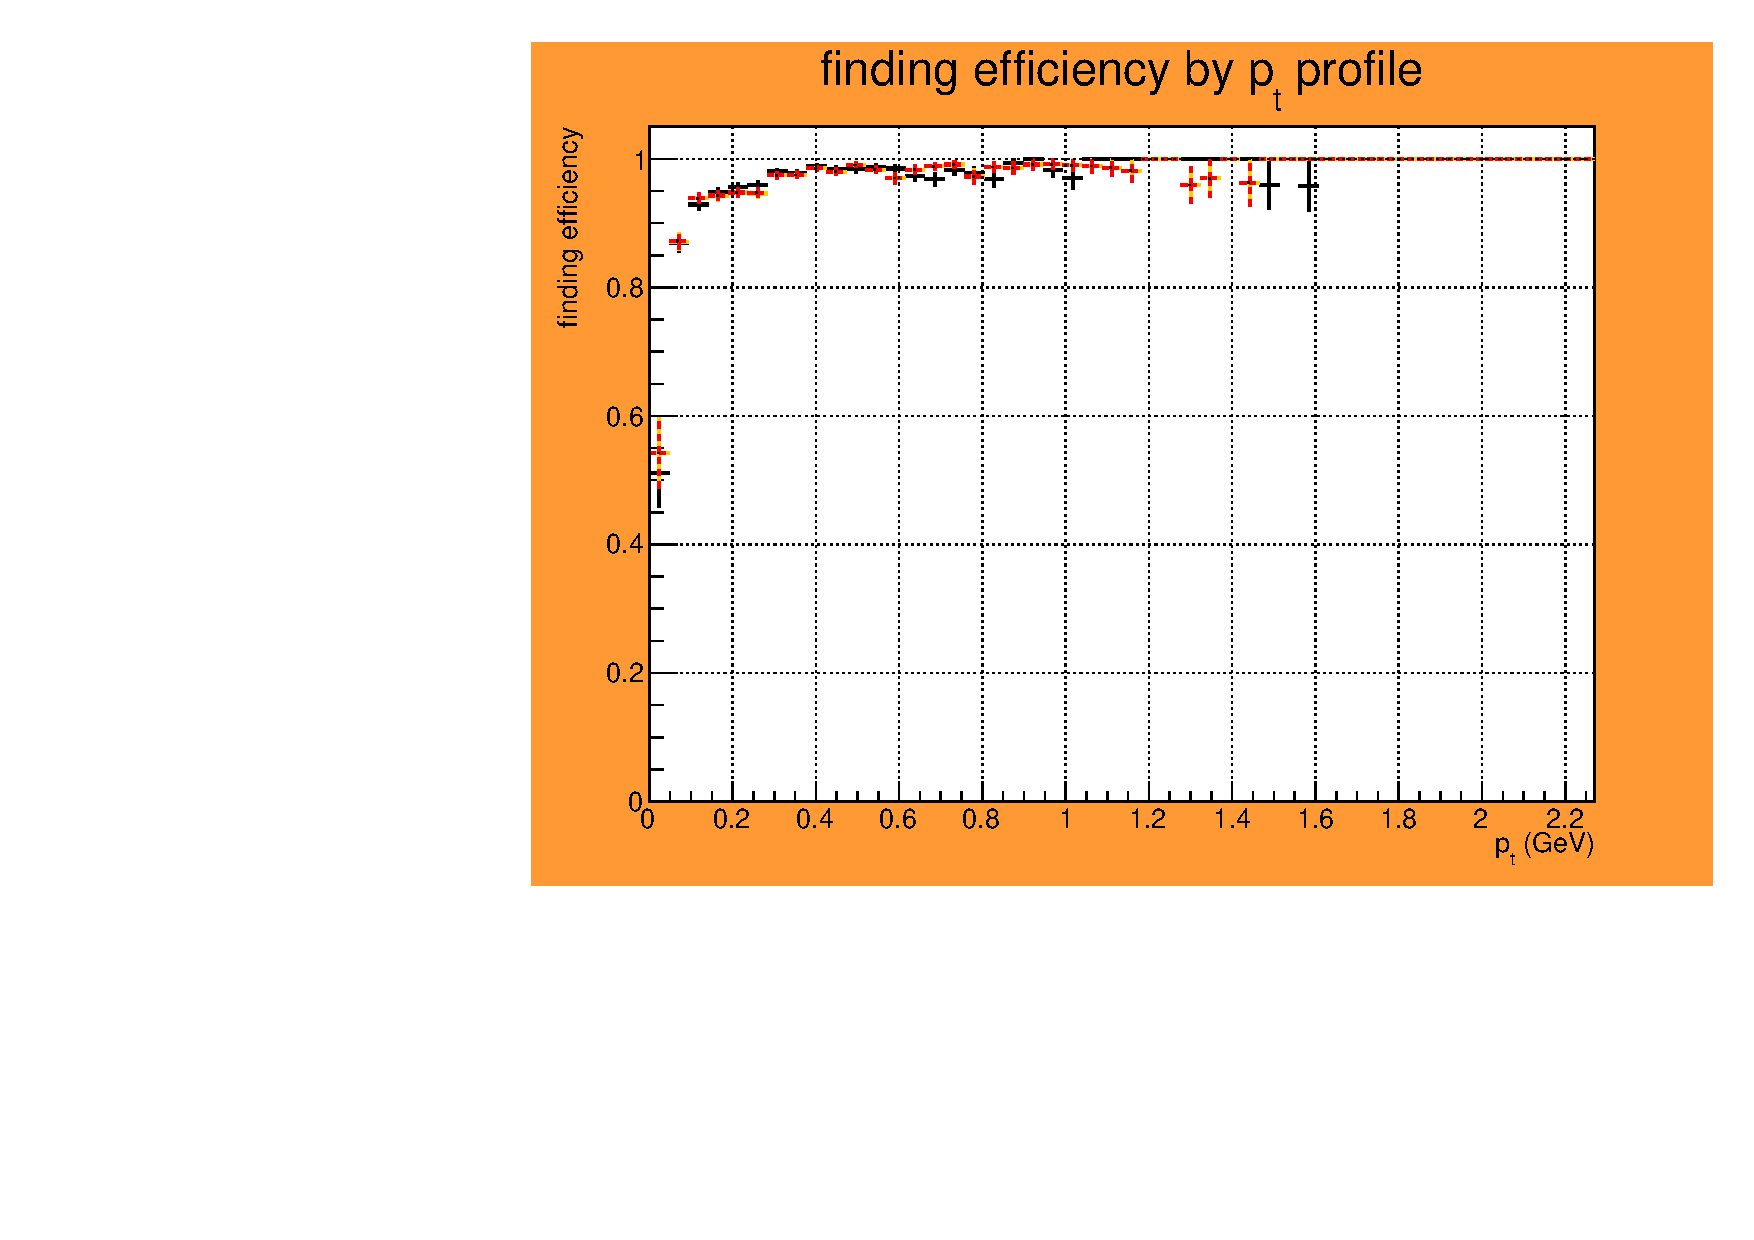
\includegraphics[width=\textwidth]{./figures/FullTrackingValidation_Full_finding_efficiency_by_p_t.pdf}
\end{center}
\end{frame}
\end{document}